\documentclass[10pt,a4paper]{article}

% ── Packages ──────────────────────────────────────────────
\usepackage[margin=1.4cm, top=1.1cm, bottom=1.1cm]{geometry}
\usepackage[dvipsnames,table]{xcolor}
\usepackage{tikz}
\usepackage[T1]{fontenc}
\usepackage{enumitem}
\usepackage{tabularx}
\usepackage{booktabs}
\usepackage{multicol}
\usepackage{fancyhdr}
\usepackage{graphicx}
\usepackage{hyperref}
\usepackage{sourcecodepro}
\usepackage{microtype}
\usepackage{titlesec}
\usepackage{parskip}
\usepackage{dashrule}
\usepackage{amsmath}

% ── Colors ────────────────────────────────────────────────
\definecolor{molpurple}{HTML}{7C3AED}
\definecolor{molpink}{HTML}{EC4899}
\definecolor{moldark}{HTML}{1E1B2E}
\definecolor{molgray}{HTML}{6B7280}
\definecolor{mollight}{HTML}{F5F3FF}
\definecolor{molgreen}{HTML}{10B981}
\definecolor{molorange}{HTML}{F59E0B}
\definecolor{molblue}{HTML}{3B82F6}

% ── Hyperref ──────────────────────────────────────────────
\hypersetup{
  colorlinks=true,
  linkcolor=molpurple,
  urlcolor=molpurple,
  pdftitle={MOL Language — Technical Datasheet},
  pdfauthor={CruxLabx / IntraMind}
}

% ── Section Styling ───────────────────────────────────────
\titleformat{\section}{\normalsize\bfseries\color{molpurple}}{\thesection}{0.5em}{}[\vspace{-0.3em}\textcolor{molpurple}{\rule{\linewidth}{0.4pt}}]
\titlespacing{\section}{0pt}{0.4em}{0.15em}

% ── Header / Footer ──────────────────────────────────────
\pagestyle{fancy}
\fancyhf{}
\renewcommand{\headrulewidth}{0pt}
\fancyfoot[L]{\footnotesize\color{molgray}\textcopyright\ 2026 CruxLabx / IntraMind. All rights reserved.}
\fancyfoot[R]{\footnotesize\color{molgray}MOL v0.3.0 $\cdot$ \thepage/2}

% ── Compact Lists ─────────────────────────────────────────
\setlist[itemize]{nosep, leftmargin=1.2em, label=\textcolor{molpurple}{\textbullet}}

% ── Commands ──────────────────────────────────────────────
\newcommand{\code}[1]{\texttt{\small\color{molpurple}#1}}
\newcommand{\badge}[2]{\tikz[baseline=(n.base)]{\node[fill=#1,rounded corners=2pt,inner sep=2pt,text=white,font=\scriptsize\bfseries](n){#2};}}
\newcommand{\stat}[2]{\begin{center}\textcolor{molpurple}{\LARGE\bfseries #1}\\[-2pt]{\scriptsize\color{molgray}#2}\end{center}}

\begin{document}

% ══════════════════════════════════════════════════════════
%  PAGE 1 — HEADER + OVERVIEW
% ══════════════════════════════════════════════════════════

% ── Title Block ───────────────────────────────────────────
\begin{tikzpicture}[remember picture, overlay]
  \fill[moldark] (current page.north west) rectangle ([yshift=-3.2cm]current page.north east);
  \node[anchor=west, text=white, font=\fontsize{32}{36}\selectfont\bfseries] at ([xshift=1.5cm, yshift=-1.3cm]current page.north west) {MOL};
  \node[anchor=west, text=molpink, font=\large] at ([xshift=5.5cm, yshift=-1.15cm]current page.north west) {The Cognitive Programming Language};
  \node[anchor=west, text=white!70, font=\small] at ([xshift=1.5cm, yshift=-2.0cm]current page.north west) {Native pipeline operators \textbar\ Auto-tracing \textbar\ AI domain types \textbar\ RAG built-in};
  \node[anchor=west, font=\scriptsize] at ([xshift=1.5cm, yshift=-2.7cm]current page.north west) {%
    \badge{molpurple}{v0.3.0}\;\;%
    \badge{molgreen}{68 Tests Passing}\;\;%
    \badge{molorange}{90+ Stdlib Functions}\;\;%
    \badge{molblue}{Python 3.10+}%
  };
\end{tikzpicture}

\vspace{2.8cm}

% ── What is MOL? ──────────────────────────────────────────
\section*{\hspace{-0.1em}What is MOL?}
\vspace{-0.3em}

\textbf{MOL} (Mind-Oriented Language) is the \textbf{first programming language} with native pipeline operators and automatic execution tracing — purpose-built for AI/RAG pipelines, cognitive computing, and data processing. Created by \textbf{Mounesh Kodi} for \textbf{IntraMind} at \textbf{CruxLabx}.

\vspace{0.15em}
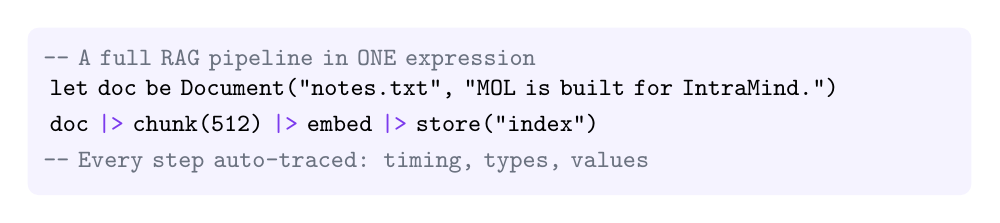
\begin{tikzpicture}
\node[fill=mollight, rounded corners=4pt, inner sep=8pt, text width=\linewidth-20pt, font=\ttfamily\small] {%
\textcolor{molgray}{-{}- A full RAG pipeline in ONE expression}\\
\textbf{let} doc \textbf{be} Document("notes.txt", "MOL is built for IntraMind.")\\[2pt]
doc \textcolor{molpurple}{\textbf{|>}} chunk(512) \textcolor{molpurple}{\textbf{|>}} embed \textcolor{molpurple}{\textbf{|>}} store("index")\\[2pt]
\textcolor{molgray}{-{}- Every step auto-traced: timing, types, values}
};
\end{tikzpicture}

% ── Stats Row ─────────────────────────────────────────────
\vspace{0.1em}
\begin{minipage}[t]{0.19\linewidth}\stat{90+}{Stdlib Functions}\end{minipage}
\begin{minipage}[t]{0.19\linewidth}\stat{8}{Domain Types}\end{minipage}
\begin{minipage}[t]{0.19\linewidth}\stat{33}{AST Nodes}\end{minipage}
\begin{minipage}[t]{0.19\linewidth}\stat{68}{Tests Passing}\end{minipage}
\begin{minipage}[t]{0.19\linewidth}\stat{2}{Transpile Targets}\end{minipage}

% ── Why MOL? ──────────────────────────────────────────────
\section*{Why MOL?}
\vspace{-0.2em}

\renewcommand{\arraystretch}{1.15}
\begin{tabularx}{\linewidth}{@{}l X X@{}}
\toprule
\textbf{Problem} & \textbf{Python / JS} & \textbf{MOL} \\
\midrule
Pipeline Debugging & \code{print()} everywhere & \code{|>} auto-traces every step \\
Data Flow & No pipe operator & \code{|>} left-to-right flow \\
AI Type Safety & Generic dicts & Native \code{Thought}, \code{Document}, \code{Embedding} \\
RAG Boilerplate & 50+ lines setup & One expression \\
Safety Rails & Hope for the best & \code{guard} + \code{access} control \\
Portability & Rewrite per language & Transpiles to Python \& JS \\
\bottomrule
\end{tabularx}

% ── Key Features (two columns) ────────────────────────────
\section*{Key Features}
\vspace{-0.2em}

\begin{multicols}{2}
\textbf{\color{molpurple}Pipeline Operator \code{|>}}
\begin{itemize}
  \item Data flows left $\to$ right through functions
  \item Auto-tracing at 3+ stages (timing, types)
  \item Named pipelines with \code{pipeline} keyword
  \item User functions as pipe stages
\end{itemize}

\textbf{\color{molpurple}Domain Types}
\begin{itemize}
  \item \textbf{Core:} Thought, Memory, Node, Stream
  \item \textbf{RAG:} Document, Chunk, Embedding, VectorStore
  \item Field access, methods, constructors
  \item Type annotations with enforcement
\end{itemize}

\columnbreak

\textbf{\color{molpurple}90+ Standard Library}
\begin{itemize}
  \item Functional: map, filter, reduce, flatten, zip
  \item Math/Stats: mean, median, stdev, sin, cos, log
  \item Strings: format, pad, starts\_with, index\_of
  \item Hashing: SHA-256, UUID, Base64
  \item Random, sorting, binary search
\end{itemize}

\textbf{\color{molpurple}Safety \& Tooling}
\begin{itemize}
  \item \code{guard} assertions with messages
  \item Access control (SecurityContext)
  \item CLI: run, parse, transpile, REPL
  \item VS Code extension (syntax, snippets)
  \item Transpiles to Python \& JavaScript
\end{itemize}
\end{multicols}

% ══════════════════════════════════════════════════════════
%  PAGE 2 — REFERENCE
% ══════════════════════════════════════════════════════════
\newpage

% ── Language at a Glance ──────────────────────────────────
\section*{Language at a Glance}
\vspace{-0.3em}

\begin{multicols}{2}

\textbf{\color{molpurple}Variables \& Types}
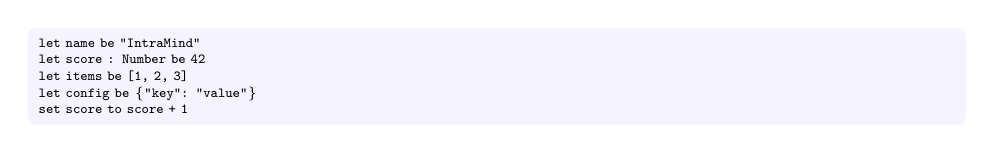
\begin{tikzpicture}
\node[fill=mollight, rounded corners=3pt, inner sep=4pt, text width=\linewidth-14pt, font=\ttfamily\tiny] {%
\textbf{let} name \textbf{be} "IntraMind"\\
\textbf{let} score : Number \textbf{be} 42\\
\textbf{let} items \textbf{be} [1, 2, 3]\\
\textbf{let} config \textbf{be} \{"key": "value"\}\\
\textbf{set} score \textbf{to} score + 1
};
\end{tikzpicture}

\vspace{0.15em}
\textbf{\color{molpurple}Control Flow}
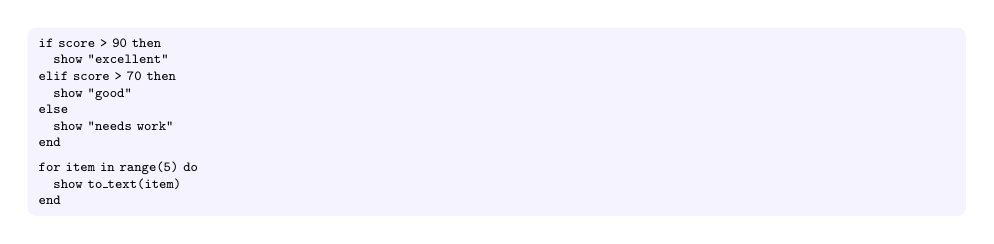
\begin{tikzpicture}
\node[fill=mollight, rounded corners=3pt, inner sep=4pt, text width=\linewidth-14pt, font=\ttfamily\tiny] {%
\textbf{if} score > 90 \textbf{then}\\
\quad \textbf{show} "excellent"\\
\textbf{elif} score > 70 \textbf{then}\\
\quad \textbf{show} "good"\\
\textbf{else}\\
\quad \textbf{show} "needs work"\\
\textbf{end}\\[3pt]
\textbf{for} item \textbf{in} range(5) \textbf{do}\\
\quad \textbf{show} to\_text(item)\\
\textbf{end}
};
\end{tikzpicture}

\columnbreak

\textbf{\color{molpurple}Functions \& Pipelines}
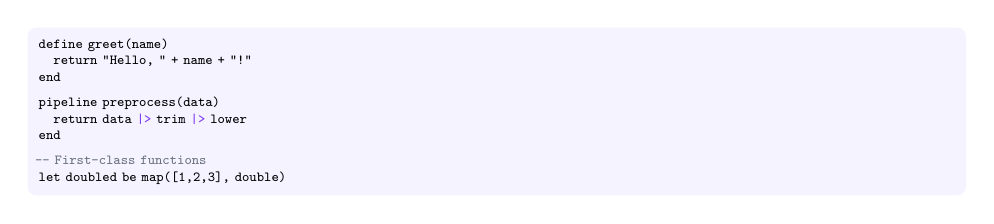
\begin{tikzpicture}
\node[fill=mollight, rounded corners=3pt, inner sep=4pt, text width=\linewidth-14pt, font=\ttfamily\tiny] {%
\textbf{define} greet(name)\\
\quad \textbf{return} "Hello, " + name + "!"\\
\textbf{end}\\[3pt]
\textbf{pipeline} preprocess(data)\\
\quad \textbf{return} data \textcolor{molpurple}{\textbf{|>}} trim \textcolor{molpurple}{\textbf{|>}} lower\\
\textbf{end}\\[3pt]
\textcolor{molgray}{-{}- First-class functions}\\
\textbf{let} doubled \textbf{be} map([1,2,3], double)
};
\end{tikzpicture}

\vspace{0.15em}
\textbf{\color{molpurple}Guards \& Safety}
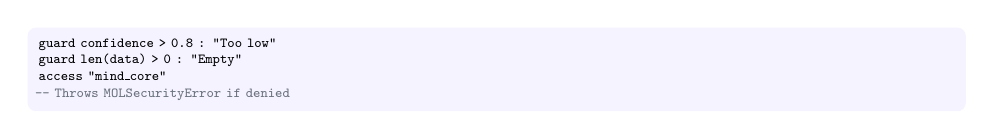
\begin{tikzpicture}
\node[fill=mollight, rounded corners=3pt, inner sep=4pt, text width=\linewidth-14pt, font=\ttfamily\tiny] {%
\textbf{guard} confidence > 0.8 : "Too low"\\
\textbf{guard} len(data) > 0 : "Empty"\\
\textbf{access} "mind\_core"\\
\textcolor{molgray}{-{}- Throws MOLSecurityError if denied}
};
\end{tikzpicture}

\end{multicols}

% ── Standard Library Reference ────────────────────────────
\section*{Standard Library (90+ Functions) \& Domain Types}
\vspace{-0.3em}

{\scriptsize
\renewcommand{\arraystretch}{1.0}
\begin{tabularx}{\linewidth}{@{}l X@{}}
\toprule
\textbf{Category} & \textbf{Functions} \\
\midrule
\textbf{General} & len, type\_of, to\_text, to\_number, range, abs, round, sqrt, max, min, sum, print \\
\textbf{Functional} & map, filter, reduce, flatten, unique, zip, enumerate, count, find, find\_index, take, drop, group\_by, chunk\_list, every, some \\
\textbf{Math} & floor, ceil, log, sin, cos, tan, pi, e, pow, clamp, lerp \\
\textbf{Statistics} & mean, median, stdev, variance, percentile \\
\textbf{Collections} & sort, sort\_by, sort\_desc, binary\_search, reverse, push, pop, keys, values, contains, join, slice \\
\textbf{Strings} & split, upper, lower, trim, replace, starts\_with, ends\_with, pad\_left, pad\_right, repeat, char\_at, index\_of, format \\
\textbf{Hash / Encode} & hash (SHA-256/MD5/SHA-1/SHA-512), uuid, base64\_encode, base64\_decode \\
\textbf{Random} & random, random\_int, shuffle, sample, choice \\
\textbf{Map Utils} & merge, pick, omit \quad\textbar\quad \textbf{Type Checks:} is\_null, is\_number, is\_text, is\_list, is\_map \\
\textbf{RAG Pipeline} & load\_text, chunk, embed, store, retrieve, cosine\_sim, think, recall, classify, summarize \\
\textbf{Debug} & display, tap, assert\_min, assert\_not\_null, inspect, to\_json, from\_json, clock, wait \\
\bottomrule
\end{tabularx}
}

\vspace{0.3em}
{\scriptsize
\renewcommand{\arraystretch}{1.0}
\begin{tabularx}{\linewidth}{@{}l l X l@{}}
\toprule
\textbf{Type} & \textbf{Category} & \textbf{Purpose} & \textbf{Constructor} \\
\midrule
Thought & Core & Cognitive unit with confidence & \code{Thought("idea", 0.9)} \\
Memory & Core & Key-value with decay & \code{Memory("key", value)} \\
Node & Core & Neural graph vertex & \code{Node("label", 0.5)} \\
Stream & Core & Real-time data buffer & \code{Stream("feed")} \\
\midrule
Document & RAG & Text with source metadata & \code{Document("file", "text")} \\
Chunk & RAG & Text fragment & \code{Chunk("text", 0, "src")} \\
Embedding & RAG & 64-dim vector (deterministic) & \code{Embedding("text", "model")} \\
VectorStore & RAG & In-memory vector index & Created via \code{store()} \\
\bottomrule
\end{tabularx}
}

% ── CLI + Architecture ────────────────────────────────────
\section*{CLI \& Architecture}
\vspace{-0.3em}

\begin{multicols}{2}

\textbf{\color{molpurple}CLI Commands}
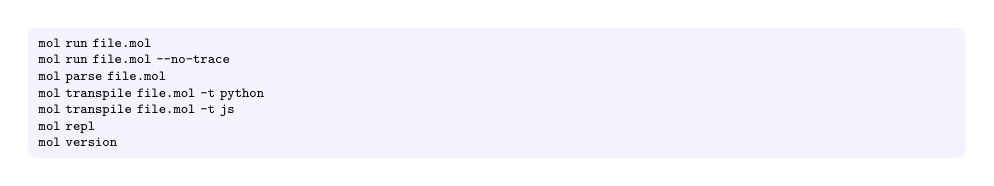
\begin{tikzpicture}
\node[fill=mollight, rounded corners=3pt, inner sep=4pt, text width=\linewidth-14pt, font=\ttfamily\tiny] {%
mol run file.mol\\
mol run file.mol -{}-no-trace\\
mol parse file.mol\\
mol transpile file.mol -t python\\
mol transpile file.mol -t js\\
mol repl\\
mol version
};
\end{tikzpicture}

\columnbreak

\textbf{\color{molpurple}Architecture}
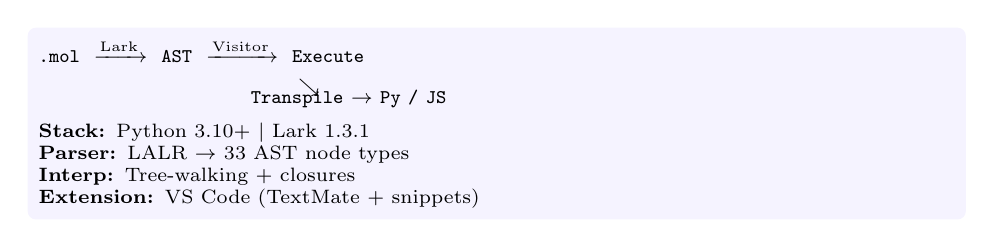
\begin{tikzpicture}
\node[fill=mollight, rounded corners=3pt, inner sep=4pt, text width=\linewidth-14pt, font=\scriptsize] {%
\texttt{.mol} $\;\xrightarrow{\text{\tiny Lark}}\;$ \texttt{AST} $\;\xrightarrow{\text{\tiny Visitor}}\;$ \texttt{Execute}\\[3pt]
\hspace{3.2cm} $\searrow$\\[-4pt]
\hspace{2.6cm} \texttt{Transpile} $\to$ \texttt{Py / JS}\\[4pt]
\textbf{Stack:} Python 3.10+ \textbar\ Lark 1.3.1\\
\textbf{Parser:} LALR $\to$ 33 AST node types\\
\textbf{Interp:} Tree-walking + closures\\
\textbf{Extension:} VS Code (TextMate + snippets)
};
\end{tikzpicture}

\end{multicols}

% ── Version + Roadmap ─────────────────────────────────────
\section*{Version History \& Roadmap}
\vspace{-0.3em}

\renewcommand{\arraystretch}{1.05}
\begin{tabularx}{\linewidth}{@{}l l l X@{}}
\toprule
\textbf{Version} & \textbf{Date} & \textbf{Status} & \textbf{Highlights} \\
\midrule
v0.1.0 & 2026-02-08 & \badge{molgreen}{Done} & Grammar, AST, interpreter, 4 domain types, CLI, transpiler, 30+ stdlib \\
v0.2.0 & 2026-02-09 & \badge{molgreen}{Done} & Pipeline \code{|>}, auto-tracing, guard, 4 RAG types, 15 RAG functions \\
v0.3.0 & 2026-02-10 & \badge{molgreen}{Done} & 42 new algorithms, 90+ stdlib, callable functions, documentation \\
v0.4.0 & — & \badge{molorange}{Next} & Sovereign AI — agent blocks, model registry, knowledge graph \\
v0.5.0 & — & \badge{molgray}{Planned} & Async pipelines, real DB integration (FAISS/Qdrant), HTTP server \\
v1.0.0 & — & \badge{molblue}{Vision} & Package manager, playground, debugger, cloud deployment \\
\bottomrule
\end{tabularx}

\vspace{0.3em}
\begin{center}
\hdashrule[0.5ex]{0.5\linewidth}{0.4pt}{2pt}\\[0.5em]
{\large\bfseries\color{moldark} Built for IntraMind by CruxLabx}\\[0.2em]
{\color{molgray}\small Creator: Mounesh Kodi \quad$\cdot$\quad \url{https://github.com/crux-ecosystem/mol-lang}}
\end{center}

\end{document}
